\documentclass[12pt]{article}
\usepackage[utf8]{inputenc}
\usepackage{graphicx}
\usepackage[serbian]{babel}

\title{Korisni alati za programiranje Android aplikacija}
\author{Danilo Nikolaš, Luka Nedeljković, Nemanja Kelečević, Ivan Vlahović}
\date{15. novembar 2022.}

\begin{document}

\maketitle
\tableofcontents
\pagebreak

\section{Uvod}
Poslednjih godina prisutan je sve veći broj aplikacija i okruženja za android, koje pružaju razne mogućnosti.
Pomenute aplikacije mogu pomoći, kako početnicima da savladaju prve korake u programiranju, tako i iskusnijim programerima da usavrše svoje veštine na efikasan i zabavan nacin.
U narednom tekstu predstavićemo aplikacije koje su nam se učinile kao najbolji izbor, medju njima su Android Studio,Unity 3D... \

\section{Android Studio}
Android Studio je jedan od najzastupljenijih i najbitnijih alata za Android programere. To je \textbf{integrisano razvojno okruženje} (IDE) za Android, zasnovano na softveru JetBrains IntelliJ IDEA.  \\
\hspace*{1cm}Službeni programski jezik je \textbf{Java}, ali su takodje podržani C++, a i od nedavno Kotlin. Razvojno okruženje poseduje kompajler koji omogućava stvaranje APK datoteka, XML uređivač, kao i funkciju za "prikaz dizajna" pomoću koje vizuelnim putem omogućava organizovanje elemenata na ekranu. \\
\hspace*{1cm}Android Studio nudi kompletan set dodatnih alata koji programeri mogu efikasno da iskoriste, kao što su AVD Manager, Android Debug Bridge, monitor za praćenje performansi itd.\\
Neke od prednosti Android Studia:-
\begin{itemize}
\item{Veoma brzo i efikasno pokretanje aplikacije}
\item{Inteligentno uredjivanje koda} 
\item{Emulator sa mnogo mogućnosti}
\item{Može se koristiti za sve android uređaje}
\end{itemize}

\begin{figure}[ht!]
    \centering
    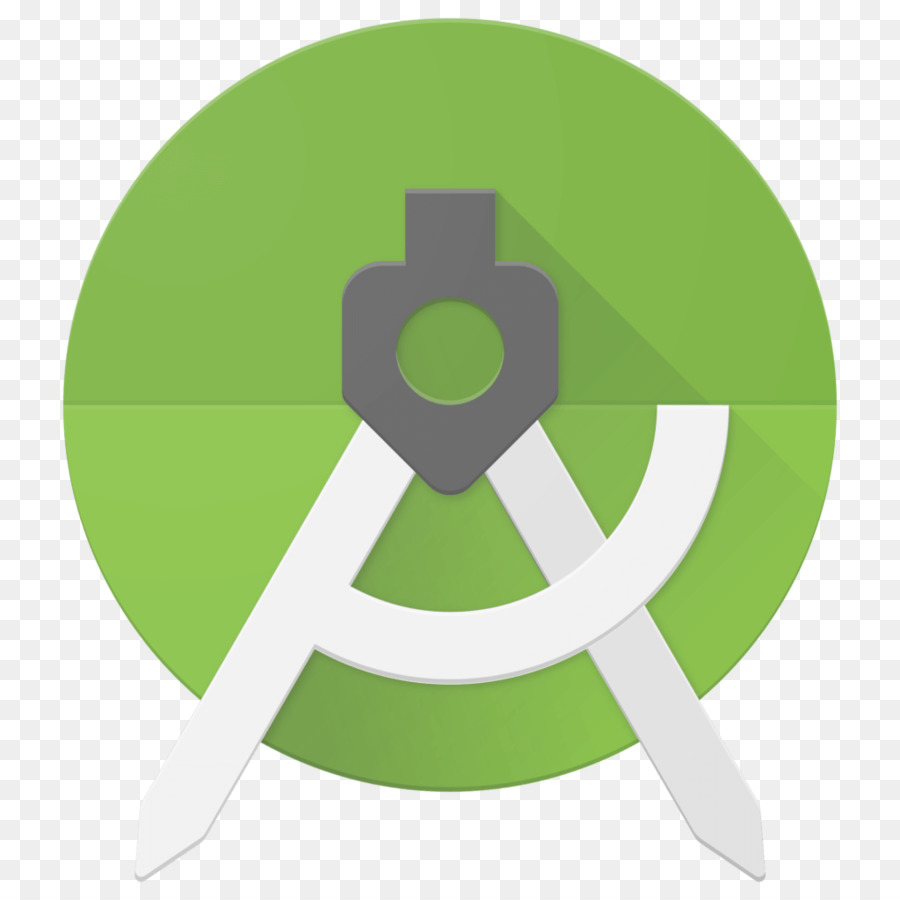
\includegraphics[scale=0.05]{android_studio_logo.jpg}
    \caption{Android Studio logo}
\end{figure}
\subsection{Neki dodatni alati Android Studia}
Alat AVD Manager (Android virtualni uređaj) je uključen u Android Studio i u osnovi je emulator koji omogućava pokretanje Android aplikacija na računaru. Zbog toga je vrlo koristan alat jer omogućava brzo testiranje aplikacija bez potrebe za instaliranjem na fizičke uređaje. Pored toga, omogućava simulaciju različitih veličina ekrana, specifikacija, verzija Androida ... Sve ovo i još više omogućava vam optimizaciju aplikacije za njeno izvršavanje na bilo kojem uređaju.

Android Debug Bridge (ADB) je još jedan od korisnih alata Android Studia. U suštini, ovaj alat omogućava terminalni interfejs za interakciju sa telefonom. Kako je Android platforma bazirana na Linuxu, terminalni pristup je jedini način dobijanja admin pristupa. ADB omogućuje most između uređaja i kompjutera.

\begin{figure}[ht!]
    \centering
    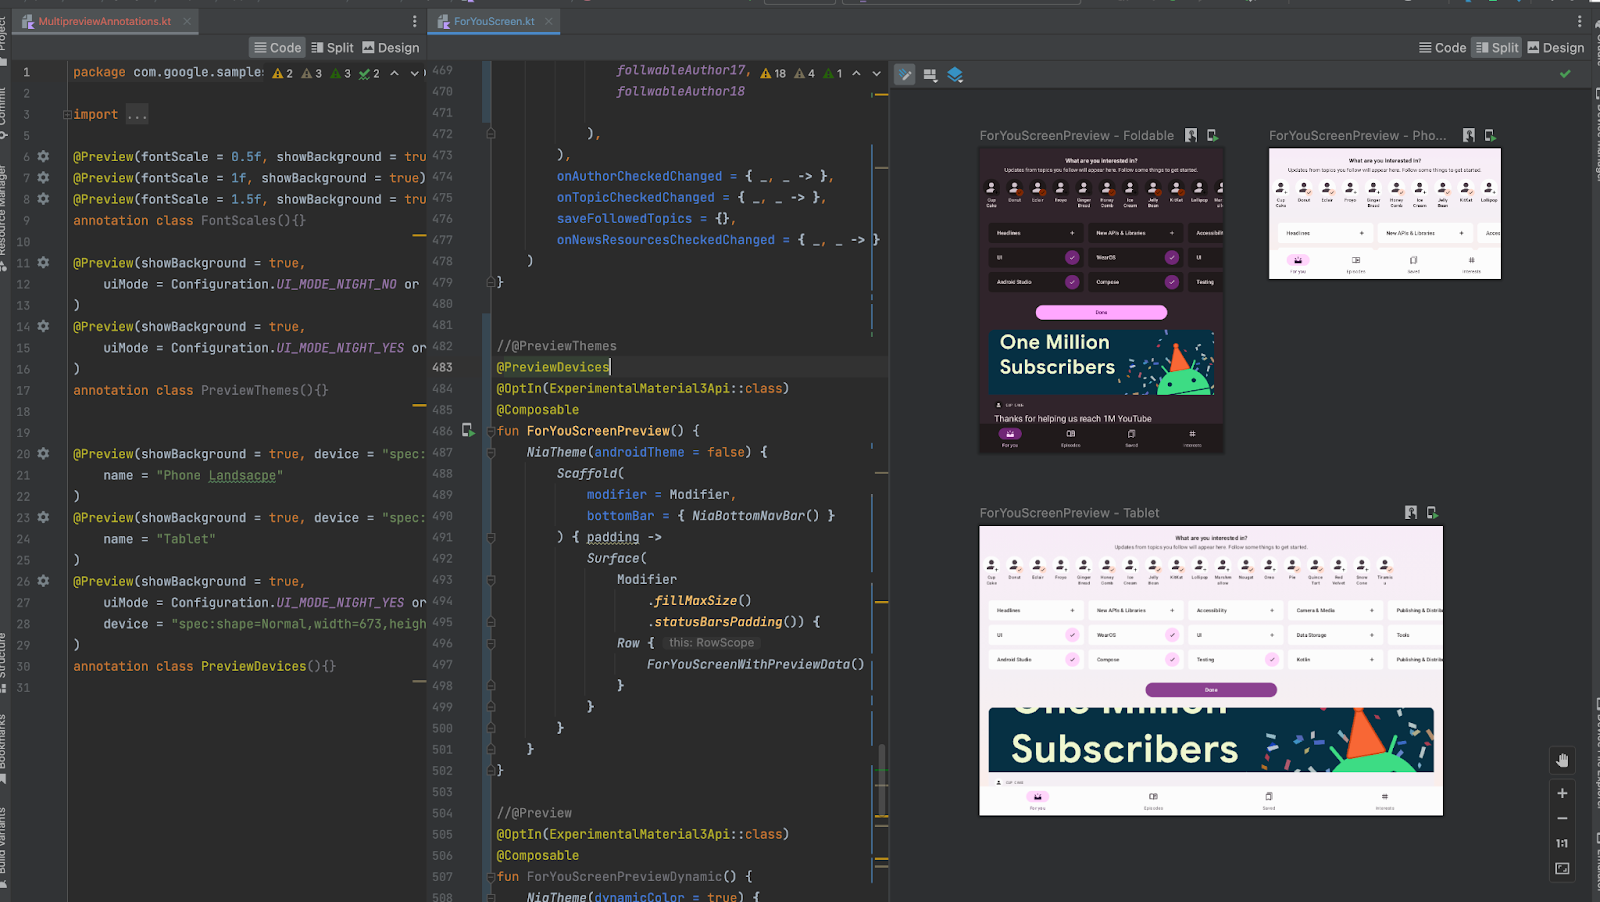
\includegraphics[scale=0.3]{android_studio_interface.png}
    \caption{Razvojno okruženje Android Studia}
\end{figure}

\section{Unity 3D}

Unity 3D je viseplatformsko okruzenje za razvoj igara sa ugradjenim IDE (Integrisano razvojno okruzenje) – softverska aplikacija koja pruza pogodnosti programerima pri razvoju softvera. IDE se sastoji od uredjivaca koda, ispravljaca gresaka I takodje poseduje algoritme automatizacije koda sto 
znatno olaksava rad programerima.

Iako je prva verzija unity-a, predstavljena na Apple konferenciji “Worldwide Developers Conference” 2005. godine, prvobitno bila namenjena da funkcionise na Mac racunarima, vremenom se razvila I postula dostupna za sve platforme. 

\begin{table}[ht!]
\begin{tabular}{|l|l|}
\hline
\multicolumn{1}{|c|}{\textbf{Unity 2.0 (2007)}} & Olaksan rad vise programera na istom projektu.\\ \hline
\textbf{Unity 3.0 (2010)}                       & Poboljsane graficke perfomanse za Desktop racunare.                               \\ \hline
\textbf{Unity 4.0 (2012)}                       & Podrska za Adobe Flash, saradnja sa Facebook-om. \\ \hline
\textbf{Unity 2017}                             & Poboljsan rad sa animacijama i kamerama. \\ \hline
\end{tabular}
\end{table}

Unity razvojno okruzenje koristi jezik C# kao primarni programski jezik.
Kako je poznavanje jezika C# I njegovih funkcionalnosti osnova programiranja I kako vecina programera jako dobro poznaje ovaj jezik, sa lakocom se moze naviknuti na rad u Unity-ju. Takodje, jezik C# ima veoma veliku zajednicu pa se moze ocekivati da je problem sa kojim se korisnik srece vec obradjen negde u okviru ove zajednice. Samim tim programer ima veliku podrsku I literaturu koja mu je dostupna pri razvoju softvera u ovom okruzenju. Ucenje programiranja se zasniva na poznavanju koncepata ovog jezika, svaki pocetnik ce vrlo lako savladati principe Unity okruzenja. 

Unity 3D ima siroku primenu na velikom broju platformi.
Koju god platformu preferirali, velike su sanse da je Unity podrzava.

\begin{figure}[ht!]
    \centering
    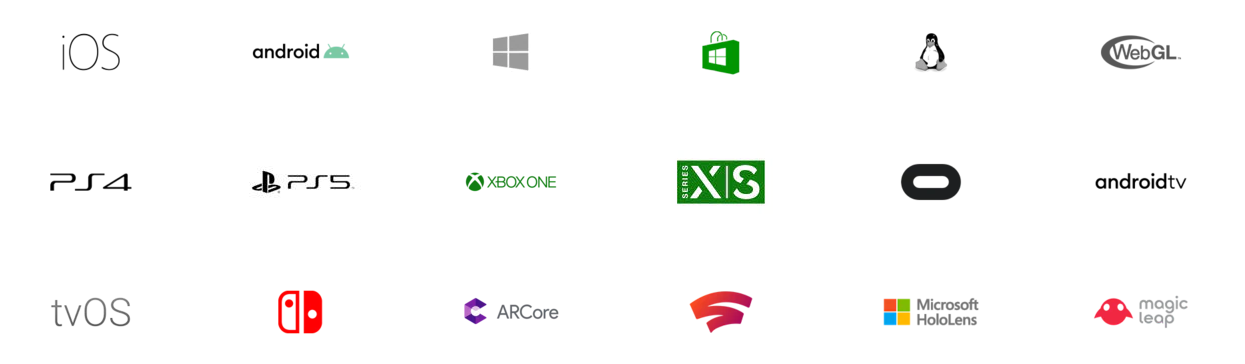
\includegraphics[scale=0.2]{platforme.png}
    \caption{Dostupne platforme}
\end{figure}


Unity podrzava I dvodimenzionalno (2D) i trodimenzionalno(3D) programiranje. Vecina programa u ovakvim situacijama favorizuje jednu opciju I naklonjena je vise ka jednoj od njih ali to nije slucaj sa Unity razvojnim okruzenjem. Postoji mnostvo alata, skracenica I opcija koje omogucavaju olaksan rad pocetnicima ali I onima sa vise iskustva. 

Interfejs Unity okruzenja je jednostavan I intuitivan. 
Ovaj interfejs svakako spada u grupu onih koji su najlaksi za koriscenje i usavrsavanje. Preglednost I jednostavnost jako su bitne karakteristike
ovog okruzenja. Takodje, programeri su u mogucnosti da izgled interfejsa i njegove pogodnosti prilagode sebi i svojim navikama jer je Unity interfejs
podlozan modifikacijama. 

Unity u okviru svog okruzenja sadrzi I \textbf{Asset Store} – platforma na kojoj programeri mogu deliti svoje kodove I biblioteke. Mnoge funkcionalnosti su dostupne potpuno besplatno, takodje programeri svoje kodove mogu I prodavati u okviru ove platforme. Pocetnici mogu koristiti ovu prodavnicu I bilbioteke ugradjene u njoj da razviju svoj softver od nule sto omogucava lakse upoznavanje sa konceptima programiranja u Unity okruzenju.
Sa druge strane, iskusniji programeri nece morati da razvijaju delove softvera koji vec postoje pa tako mogu usmeriti svoje vreme na kreiranje novog softvera.

Unity ima jos jednu pogodnost za nove korisnike - potpuno besplatne obuke na svom oficijalnom sajtu.
Bilo da se radi o apsolutnim pocetnicima ili ipak iskusnijim programerima, ove obuke svima znace jer ih uvode u temu i upoznaju sa mnogim      funkcionalnostima ovog razvojnog okruzenja.
Sve neophodne dokumentacije I interfejsi su takodje besplatni I dostupni na internetu.

\section{Unreal Engine}

\section{Basic4Android}
\hspace*{1cm} Basic4Android, poznatiji kao B4A, je alatka za brzi razvoj aplikacija na Androidu.B4A koriste na desetine hiljada programera iz celog sveta, uključujući i najveće svetske kompanije poput NASA-e, HP-a, IBM-a.
Zajedno sa B4i mogu se lako isprogramirati aplikacije i za iOS i za Android istovremeno.B4A je alternativa programiranju u Javi. Programski jezik je sličan Visual Basic-u i Visual Basic.Net -u iako je adaptiran prirodnom Android okruženju.

B4A sadrži vizuelni dizajn koji u mnogome pomaže proces pravljenja korisničkog interfejsa koji se koriste na telefonima i tabletima u različitim veličinama. Kompajlirani programi mogu se testirati u AVD Manager emulatorima, ili na pravim Android uređajima koristeći Android Debug Bridge i B4A Bridge. 
B4A generiše standardne Android aplikacije koje mogu biti postavljene na prodavnicama aplikacija poput Google Play-a, Samsung Apps-a, Amazon Appstore-a.

Aplikacije:
B4A podržava sve tipove aplikacija kao što su igrice, baze podataka, senzore i hardver.

BIBLIOTEKE:
B4A biblioteka se sastoji od dva fajla: Java fajl i XML fajl koji je obezbeđen od strane alatki B4A.
\begin{figure}[ht!]
    \centering
    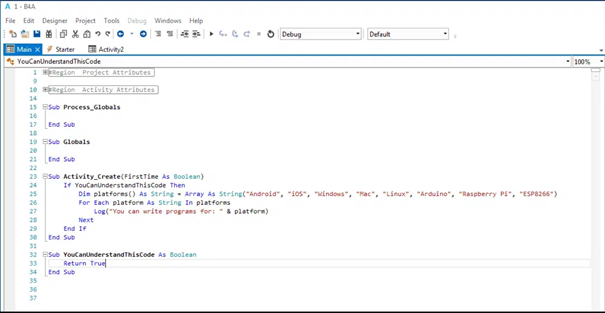
\includegraphics[scale=0.05]{b4aslika.png}
    \caption{Android Studio logo}
\end{figure}
\section{Zaključak}

Android je definitivno projekat koji mnogo obećava. Jedna od njegovih glavnih prednosti je dobra organizacija, koja ima potencijal da iskoristi svu moć i znanje zajednice otvorenog koda. Još jedna dobra stvar je uključenost velikog broja jakih kompanija u projekt, što omogućuje jako brzo širenje.
Brži razvoj, kao posledica dobre organizacije, povlači za sobom unapređivanje svih aspekata projekta.
Svako može učestvovati,što će dodatno podsticati inovacije i ubrzati razvoj.
Svakodnevno se platforma tehnički usavršava i unapređuje od strane nezavisnih
proizvođača. Android je vodeći operativni sistem za mobilne telefone i predpostavlja se da će
i u budućnosti biti u vrhu i doneti mnoštvo inovacija.

\pagebreak
\begin{thebibliography}{}
\bibitem
\bibitem
\bibitem
\bibitem
\bibitem https://www.androidsis.com/bs/najbolji-alati-za-programere-android-aplikacija/
\bibitem https://androidayuda.com/bs/android-studio/
\end{thebibliography}

\end{document}
